\part{Concept}%

\chapter{Interaction of Light and Matter}
Traditionally cells have been studied with optical light. To understand why light is a good probe to study cells, it is necessary to understand the nature of its interaction with matter. For most work described in this thesis the classical model of describing light as a wave is sufficient. This chapter will create the mathematical framework that describes how light behaves in our diffraction experiments. 

\section{Light as electromagnetic radiation}
In the 17th and 18th century it became possible for humans to generate electric charges and continuous currents [Guericke, Leiden, Volta], enabling the investigation of the phenomena of electricity and magnetism. This ultimately led to a ground-breaking work by Maxwel where he ties together the fields of magnetism, electricity, and somewhat surprisingly, optics. His results are known as the Maxwell equations:

\begin{equation} \nabla \cdot   \vec{E} = \frac{\rho}{\varepsilon_0 }\label{eq:maxlaw1}\end{equation}
\begin{equation} \nabla \cdot   \vec{B} = 0 \label{eq:maxlaw2}\end{equation}
\begin{equation} \nabla \times \vec{E} = -\frac{d\vec{B}}{dt}\label{eq:maxlaw3}\end{equation}
\begin{equation} \nabla \times \vec{B} = \mu_0 \vec{J} -\mu\varepsilon\frac{d\vec{E}}{dt}\label{eq:maxlaw4}\end{equation}

Here, $\vec{E}$ is the electric field, $\vec{B}$ is the magnetic field, $\varepsilon$ and $\mu$ are respectively the permittivity and the permeability of the material. $\rho$ is the the charge density and $\vec{J}$ describes the local current. %Equation \ref{eq:maxlaw1} shows that the electric flux
%leaving a volume is proportional to the charge inside. Equation
%\ref{eq:maxlaw2} states that the magnetic flux leaving a volume is
%always 0. This means that the north and south pole of a magnet are
%always connected, which finds its origin in the dipole moment of the
%electron itself. Equation \ref{eq:maxlaw3} shows that the voltage
%induced in a closed loop in proportional to the rate of change of the
%magnetic flux that the loop encloses. A dynamo uses this phenomena to
%generate a charge. Equation \ref{eq:maxlaw4} shows that the magnetic
%field induced around a closed loop is proportional to the electric
%current plus the rate of change in the electric field. Electric motors
%exploit this phenomena. 
An important consequence of these equations is that a moving charge will induce a magnetic field, which in its turn induces a change in the electric field, and so on.

In order to understand why these laws unify magnetism, electricity and optics, we will consider a special case: vacuum. In vacuum there are no localized charges ($\rho = 0$) and no currents ($\vec{J}=0$), which simplifies equation \ref{eq:maxlaw1} and \ref{eq:maxlaw4} to: 

\begin{equation} \nabla \cdot   \vec{E} = 0 \label{eq:maxlaw1_vac}\end{equation}
\begin{equation} \nabla \times \vec{B} = -\mu_0\varepsilon_0\frac{d\vec{E}}{dt}\label{eq:maxlaw4_vac}\end{equation}

Furthermore, experiments showed that the permittivity for vacuum, $\varepsilon_0 = 8.854\cdot10^{-12} Fm^{-1}$, and the permeability for vacuum$mu_0 = 1.257 \cdot 10^{-7} N A^{-2}$. If we now ask ourselves what the field change caused by a change in the electric field is by studying the equation $\nabla \times( \nabla \times \vec{E}) $, we can derive something quite amazing:  
\[ \nabla \times( \nabla \times \vec{E}) = \nabla (\nabla \cdot
\vec{E}) -\nabla^2 \vec{E} =-\nabla^2 \vec{E} \]
The first equality is a well known mathematical relation, and for the second equality equation \ref{eq:maxlaw1_vac} is used. 
Now lets rewrite the equation in a different way:
\[\nabla \times( \nabla \times \vec{E})=
\nabla\times(-\frac{d\vec{B}}{dt}) =
-\frac{d}{dt}(\nabla\times\vec{B})=\frac{d}{dt}(\mu_0\varepsilon_0\frac{d\vec{E}}{dt})
= \mu_0\varepsilon_0\frac{d^2\vec{E}}{dt^2}\]
In the first equality we used equation \ref{eq:maxlaw3}. In the second equality we used a general algebraic property. In the third equality we used \ref{eq:maxlaw4_vac}, and in the last equality we combined the two time derivatives. Together these equations state that:

\begin{equation}\label{eq:wave_eq}
\frac{d^2\vec{E}}{dt^2} = \frac{1}{\mu_0\varepsilon_0}\nabla^2 \vec{E} = v^2 \nabla^2 \vec{E},      v = \frac{1}{\sqrt{\mu_0\varepsilon_0}}
\end{equation}

Equation \ref{eq:wave_eq} is known as the wave equation, which is used to describe the propagation of a wave with the speed $v$. Combining this results with the experimentally determined value for $\mu_0$ and $\varepsilon_0$ shows that electromagnetic (EM) waves travel at \(3\cdot 10^8 \frac{m}{s}\), which agreed with value of the speed of light \cite{Froome1971}. This result strongly hints at the possibility that light is an electromagnetic wave. Further experiments succeeded in demonstrating the existence of electromagnetic waves with long wavelengths and showed that their properties are consistent with the properties of visible light, including their velocity. Visible light has now become part of the broader spectrum of electromagnetic radiation. Although Quantum Mechanics complicated the description of light further, as light can demonstrate particle-like behaviour under certain conditions. Many phenomena however can be described by treating light as a wave. 

\section{Photon-material interactions}
Assuming that light is electromagnetic radiation, it is easy to understand that a change in electric field will affect its propagation. There are four mechanisms through which radiation interacts with matter: photoabsorption, scattering, photo-nuclear absorption and pair production. The description of these phenomena will treat as if light will come in discrete quanta: photons. 
Photonuclear absorption and pair production only occur when matter is exposed to high energy gamma rays, and are therefore of little relevance to this thesis. Photoabsorption is facilitated primarily through a process called photoexcitation, in which an electron is excited to a higher level of energy, or possibly ionized in the case of photoionisation. Scattering can be divided into two classes: elastic scattering and inelastic scattering. Elastic scattering does not result in a change of kinetic energy of the scattering particle, nor does it change the wavelength of the radiation. Only the direction of the radiation can be changed. Inelastic scattering leads to both a change in wavelength of the radiation, and a change in kinetic energy. Photo-absorption and inelastic scattering deposit energy into the object which will lead to structural changes of the object. Elastic scattering on the other hand can be used to gain structural information about the object, without causing damage to the object. 

\subsection{Scattering by a single free electron}
The simplest example of elastic scattering is Thompson scattering from a free electron. A free electron will scatter or diffract the incoming radiation in all directions. An important physical concept for understanding scattering on a deeper level is the Lorentz force which describes the force exerted on a charged particle travelling in a electromagnetic field. 
\begin{equation}\label{eq:lorentz}
\vec{F} = q\vec{E} + q\vec{v}\times\vec{B}
\end{equation} 

From Newton's second law of motion ($\vec{F} = m \vec{a}$) it is known that force and acceleration are
proportional and parallel, thus the Lorentz force describes the acceleration of a charge in an electric and/or magnetic field. The first term of equation \ref{eq:lorentz} is also known as the Coulombic force, and shows that a charge is accelerated in the direction of an electric field. The second term shows that a moving charge is accelerated by the presence of a magnetic field in the direction that is both perpendicular to its movement and the magnetic field, given that $\vec{v}$ and $\vec{B}$ are not parallel in which case there is no acceleration.

According to classical electromagnetic theory the electric field associated with a monochromatic plane wave of amplitude $E_0$, and wavelength $\lambda$, propagating in the z-direction can be described by: 

\begin{equation}\label{eq:plane_wave}
\vec{E_{in}} = E_0 e^{-2\,\pi\ i \frac{ c t }{\lambda}}
\end{equation} 

When the oscillating electric field of the incident EM wave hits a stationary electron of mass $m_e$ and charge $e$ located at position $z = 0$, it exerts a Coulombic force on the electron which causes it to oscillate at the same frequency as the incident radiation. By Newton's second law of motion:

\begin{align}\label{eq:motion_single}
\vec{F} = m_e \vec{a}(t) =& e E_0 e^{-2\,\pi\ i \frac{ c t}{\lambda}} \\
\vec{a}(t) =& \frac{e\,E_0}{m} e^{-2\,\pi\ i \frac{c\,t}{\lambda}}
\end{align}

Here we assumed the contribution of the magnetic part of field to be negligible, as the electron will not reach a significant velocity.
An accelerated charge emits electromagnetic radiation. The oscillating electron becomes a new source of radiation that radiates spherically in all directions, at the same frequency as the incident radiation. From Maxwell's equations it follows that the electric field generated by an accelerating electron measured at point $\vec{d}$  can be described as []:

\begin{equation}\label{eq:scattering}
\vec{E_s}(\vec{d},t) = \frac{e a_\perp(t)}{4 \pi \varepsilon_0c^2d}
\end{equation}

$a_{\perp}(t)$ is the acceleration projected on a plane perpendicular to $\vec{d}$. 
\begin{equation}\label{eq:acceleration_perpendicular}
a_\perp = |\vec{a(t)}|\sin(\theta)
\end{equation}

Combining equations \ref{eq:motion_single}, \ref{eq:scattering}, and \ref{eq:acceleration_perpendicular}, we get that the instantaneous scattered field is:
\begin{equation}
E_s(\vec{d},t) = \frac{{e}^2}{4 \pi \varepsilon_0 m_e\,c^2} \frac{E_0 \sin(\theta)}{d} e^{-2\,\pi\ i \frac{|\vec{d}|}{\lambda}}
\end{equation}

The classical electron radius $r_e$ can be used to simplify the equation for the scattered field $E_s$
\begin{align*}
E_s=& - \frac{r_e\,E_0\,\sin(\theta)}{d} e^{-2\,\pi\ i \frac{|\vec{d}|}{\lambda}}\\
r_e =& \frac{e^2}{4 \pi \varepsilon_0 m_e\,c^2}    
\end{align*}


\subsection{Two-body scattering}
%\subsection{Approximations} 
If more than one electron are present the scattered waves will interfere, similar to the interference of water waves. The resulting pattern of dark and light bands is called a diffraction pattern. The first person to report this phenomenon was Grimaldi in 1660. Whether the interference is constructive of destructive depends on the optical path difference (OPD) between the scattered waves. Waves with path differences close to integer numbers of wavelengths interfere constructively, if close to half integral waves will interfere destructively. The central light band is often referred to as the zeroth diffraction order, or more colloquially as the central speckle. The light band next to it is called the first diffraction order (or first fringe), the one next to that the second order and so on. These terms will be used throughout the thesis. Figure \ref{fig:Interference} illustrates the phenomenon of interference.

\begin{figure}[h]\label{fig:Interference}
\centering 
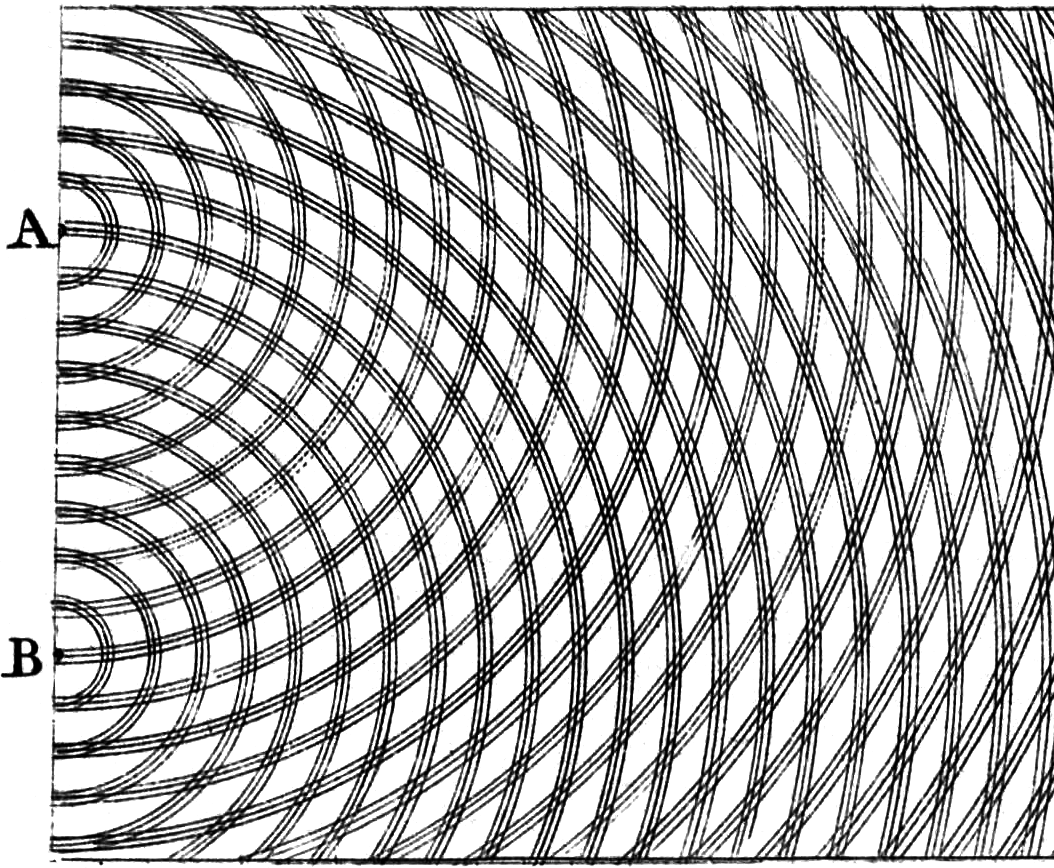
\includegraphics[width=46mm]{Young_Diffraction2.png}
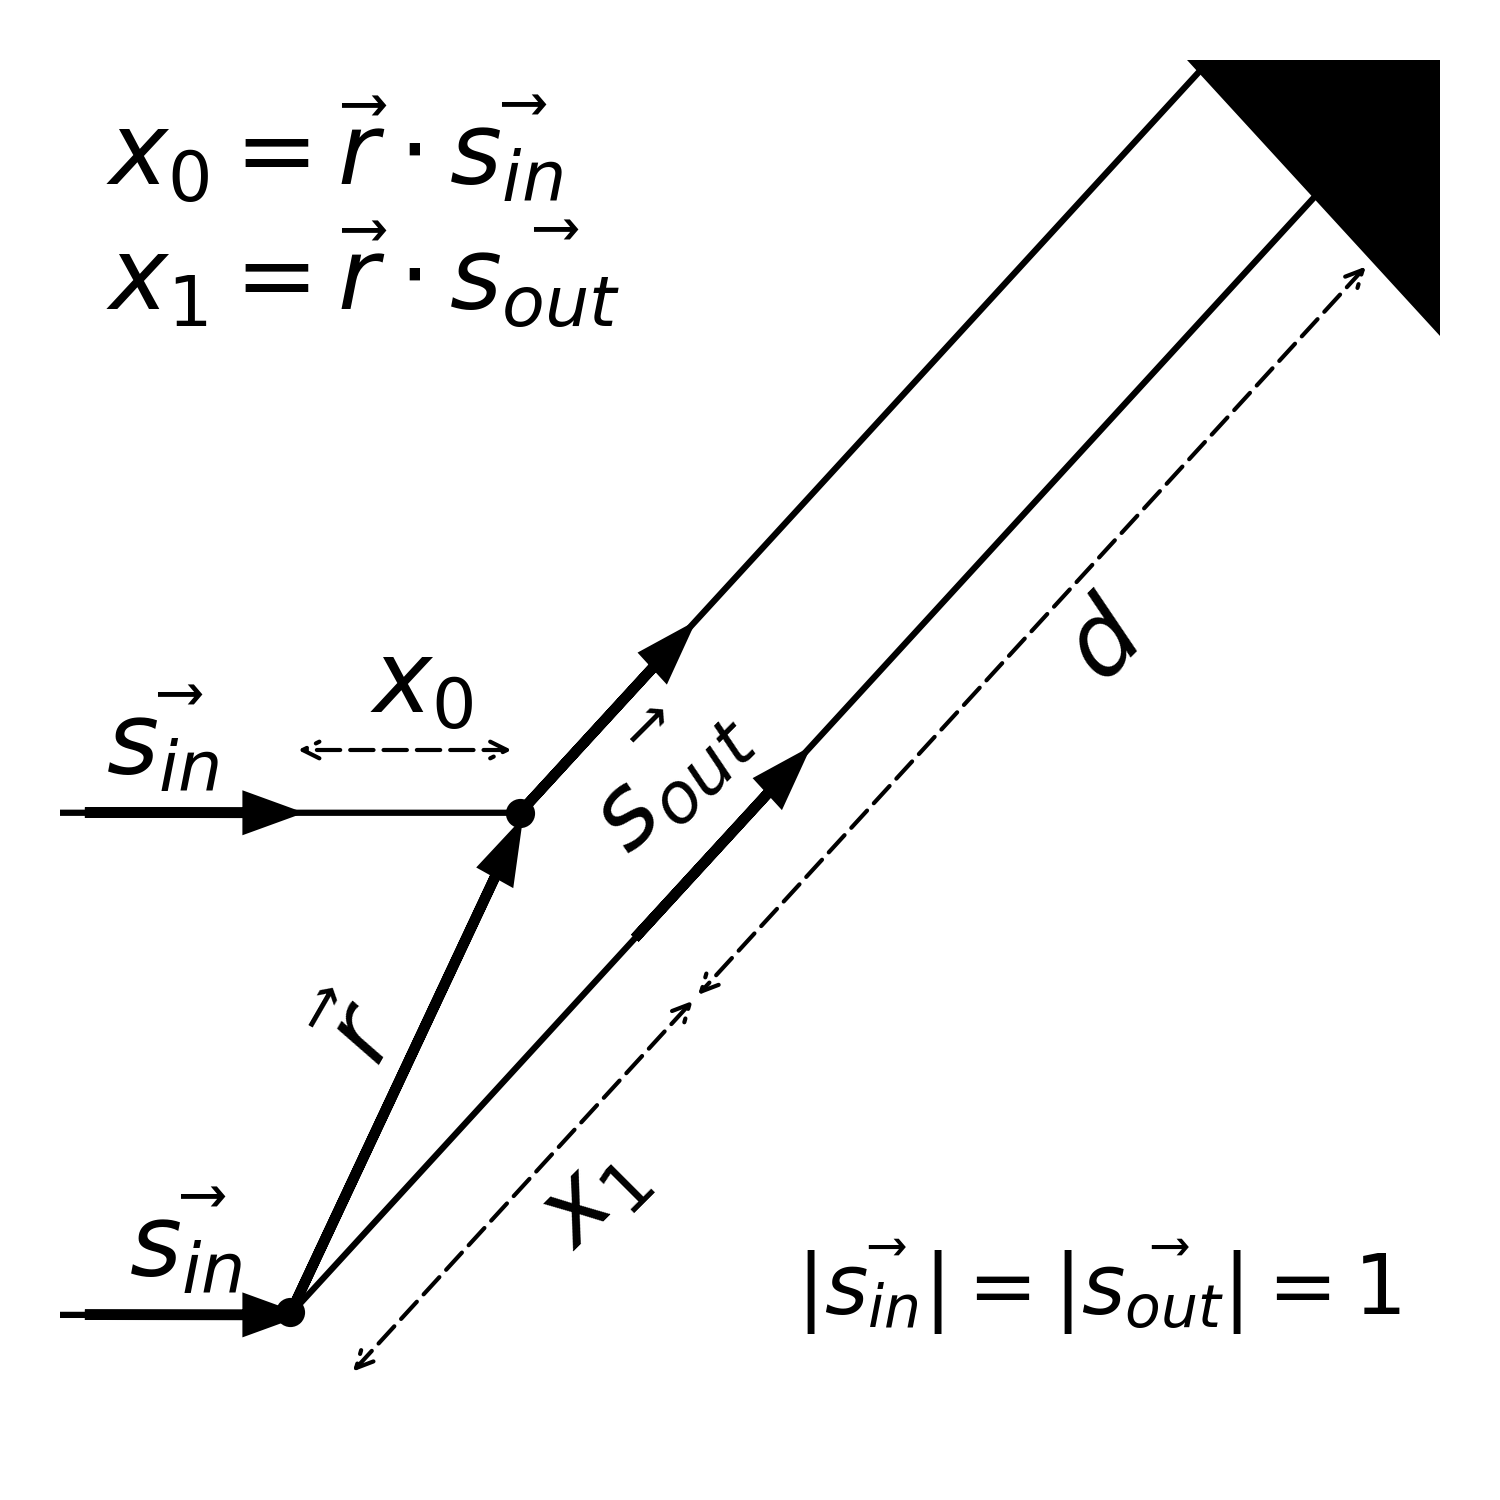
\includegraphics[width=40mm]{blah.png}

\caption{Illustration of scattering from two free-electrons A and B. a) graphic taken from Young, showing an interference pattern between two waves. b) mathematical description of the path length difference between two waves arriving at point $\vec{d}$. $\vec{s_{in}}$ and $\vec{s_{out}}$ are vectors of legnth $1/\lambda$, pointing in the direction of the incident wave and the out going wave respectively. $\vec{r}$ is a position vector describing the distance from of point A to point B. Note that in a) $x_0 = 0$.}
\end{figure}

If the diffraction pattern is measured at point \(\vec{d}\), far away from the diffracting object itself, both scattered fields have approximately the same field strength since the distance from both electrons to the detector is about equal. In Figure \ref{fig:Interference} this means that  $|\vec{d}+x_1| \approx |\vec{d}|$, and that both lines are parallel. This approximation is called the far-field approximation. The Fresnel number (FN) is used to verify the validity of the far-field approximation.
\begin{equation} 
FN = \frac{o^2}{d\lambda}
\end{equation}
where $o$ is the object size, $d$ the distance from the
object to the detector, and \(\lambda\) the
wavelength of the radiation. The far-field approximation is valid when $FN \ll 1$. All diffraction patterns discussed
in this thesis are taken in the far-field. 

The electric field at point $\vec{d}$ is given by a sum of the individual scattered electric fields:
\begin{equation}
E(\vec{d}) = E_s(\vec{d})+E_s(\vec{d}) e^{\frac{2 \pi\,i\,\Delta x}{\lambda}} 	 
\end{equation}
$\Delta x$ is the optical path difference between the two scattered waves due to the relative difference in position. $\Delta x$ can be determined by summing $x_0$ which is the path difference of the incoming radiation and $x_1$ which is the path difference of the outgoing radiation. Both $x_0$ and $x_1$ can be described using the difference vector $\vec{r}$: 
\begin{equation}
\Delta x = x_0 - x_1 =\vec{s_{out}} \cdot \vec{r}-\vec{ s_{in}}\cdot \vec{r} = (\vec{s_{out}} -\vec{s_{in}} ) \cdot \vec{r} 
\end{equation}

By defining the scattering vector $\vec{S}$
\begin{equation}
\vec{S} = \vec{s_{out}}-\vec{s_{in}}
\end{equation}
the diffraction pattern of two electrons will be :
\begin{equation}
E(\vec{d}) = E_s(\vec{d}) + E_s(\vec{d}) e^{2\,\pi\,  i\,\vec{S}\cdot\vec{r}}
\end{equation}

Important to note is that $\Delta x $ can be at most $|\vec{r}|$, the distance between the two electrons. Abbe demonstrated that in order to resolve two electrons from each other at least two diffraction orders must be captured. This usually means the zeroth and the first order. The first order start where $\Delta x > \lambda/2$. For two electrons closer than half a wavelength apart this will never be the case. This sets a physical limit to the possible details one can resolve using a regular diffraction set-up. One would not be able to use green light ($\lambda = 500\,nm$) to image objects smaller than 250 nm. For structural studies of molecules this means that in order to distinguish single atoms, X-ray radiation is required.


\subsection{Scattering from multiple electrons}
In biological particles the incoming EM radiation is scattered by many electrons. The electric field can be described as the sum of all the individual scattered fields.
\begin{equation}\label{eq:boehoe}
E(\vec{d}) = E_s(\vec{d}) \sum_{n} e^{2\,\pi\,  i\,\vec{S}\cdot\vec{r_n}}
\end{equation}

If all electrons together are assumed to form a continuous electric charge density around the many nuclei that constitute the biological particle, equation \ref{eq:boehoe}  can be written as a continuous function. 
\begin{equation}\label{eq:cont}
E(\vec{d}) = E_s(\vec{d})\int \rho(\vec{r},\lambda) \exp^{-2\pi i \,\vec{S} \cdot \vec{r}}\,d\vec{r}
\end{equation}

$\rho(\vec{r},\lambda)$ is named the scattering potential and takes the scattering strength of each nucleus into consideration. 

So far we have implicitly assumed that the scattered field will not be scattered a second time. This approximation is called the first Born approximation. We assume this to be valid for all objects smaller than a few micrometers.

We can now introduce the scattering factor $F(\vec{S})$.
\begin{equation}
F(\vec{S}) = \frac{E(\vec{d})}{E_s(\vec{d})} = F(\frac{\vec{d}}{|d|}
\end{equation}
The structure factor is independent of the distance of the detector, it only depends on the angle of measurement. Equation \ref{eq:cont} can be rewritten as:
\begin{equation}\label{eq:diff_equation}
F(\vec{S}) = \int \rho(\vec{r},\lambda) \exp^{-2\pi i \,\vec{S} \cdot \vec{r}}\,d\vec{r}
\end{equation}
This equation shows that a diffraction experiment is simply the 3D Fourier transform of the electron density evaluated at $\vec{S}$. This relation is very convenient as there is a large mathematical field describing the relations of Fourier transformations. A few of these relations are very useful to this thesis.

The Fourier shift theorem describes the change in the diffraction pattern upon object translation (i.e. shift).
\begin{equation}
\mathcal{F}(f(x+\delta x))=e^{2\pi i \delta x q} \mathcal{F}(f)
\end{equation}
The factor $e^{2 \pi i \delta x q}$ is called a 'phase-ramp'.

The Convolution theorem states that a multiplication in Fourier space is a convolution in object space (real space) and vice versa.
\begin{equation}
f(x) * g(x) = \int f(\tau)g(x-\tau)\,d\tau = \mathcal{F}^{-1} {\mathcal{F}f(x)\times\mathcal{F}g(x)}
\end{equation}

The Fourier slice theorem states that a 2D diffraction pattern is a slice through the center of the 3D fourier transform of the object.
It has thus become possible to move between diffraction pattern and electron density.


\subsection{Scattering Potential}
An important term in equation that needs further development is the scattering potential of a material $\rho(\vec{r},\lambda)$. Mathematically $\rho(\vec{r},\lambda)$ can be formulated as a function of the refractive index $n$ of a material.
\begin{equation}
\rho(\vec{r},\lambda) = \pi s_{in}^2 (( n(\vec{r},\lambda))^2 -1))
\end{equation}
$s = \frac{1}{\lambda}$

The refractive index is related to the scattering factors of the individual atoms in the material.
\begin{equation}
n = 1-\frac{r_e}{2\pi} \lambda^{2} \sum_{i} N_i f_i(0)
\end{equation}
where $r_e$ is the classical electron radius, $\lambda$ is the wavelength, $N_i$ is the number of atoms per unit volume. The complex scattering factor in the forward direction $f(0)$ can be described by: 
\begin{equation}
f(0) = f_1 + i f_2
\end{equation}
The imaginary part is derived from the atomic photoabsorption cross section and is a measure of absorption [booklet]. The real part is related to the imaginary part using the Kramers-Kronig dispersion relation [Kramers]. At high photon energies $f_1$ approaches the atomic number of the atoms. The exact value of $f_1$ and $f_2$ at different photon-energies have been determined experimentally [Henke]. 

Figure \ref{fig:waterwindow} presents the scattering factors of two elements: carbon and oxygen. The gray energy range from 282-533 eV (4.40 nm - 2.33 nm) is called the water window. In this region, and especially towards the end, oxygen atoms (thus water) are scattering significantly less than carbon atoms (i.e. organic biomolecules). The water window therefore a good candidate for imaging cells, as the contrast between two of their main constituents, water and biomolecules, is enhanced.

\begin{figure}[h]\label{fig:waterwindow}
\centering 
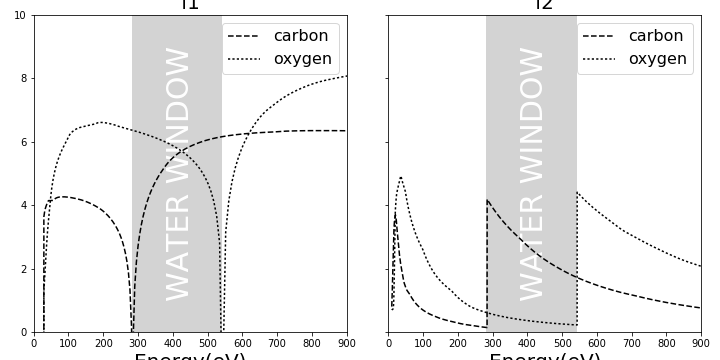
\includegraphics[width=80mm]{waterwindow.png}

\caption{Atomic scattering factors $f_1$ and $f_2$ of carbon and oxygen, as a function of photon-energy of the X-ray radiation. The region between the absorption K-edge of carbon (282 eV, 4.40 nm) and the K-edge of oxygen (533 eV, 2.33 nm) is called the water window.  The contrast between biomolecules and water is enhanced in this region, especially towards the high end of it. These wavelengths could be used for imaging living biological particles such as cells or organelles.}
\end{figure}

\section{Radiation Damage}
The previous section shows that scattering power of an body is related to the wavelength of the radiation. The shorter the wavelength the less scattering occurs. To compensate for this loss in signal, the required dose for imaging increases. Practically this means that a dose in excess of 100 MGy is required to record an interpretable signal from a living cell (a dose of 2000 Gy is already enough to kill everything that lives on earth). Unfortunately other processes of matter-radiation interaction become more abundant as well. At soft X-ray wavelengths the predominant damage process is photoionisation. Many process follow the ionization, of which non-radiative Auger decay will lead to significant radiation damage. The relation between the required dose of radiation versus the maximum tolerable dose of radiation posed a physical limit to the obtained resolution for imaging single biomolecules [Howell].

\section{Diffract-before-destroy}
An elegant solution to the problem of radiation damage came from the realization that elastic scattering occurs on a  time scale shorter than the damage processes manifest themselves structurally. This principle is of diffract-before-destroy, suggested in 2000 by Neutze et al [], was experimentally demonstrated on a silicon-nitrate sample [Chapman]. This experiment used the ultra short and extremely bright pulses from the first x-ray free-electron laser to outrun key damage processes. Although the pulse literally obliterated the sample, enough structural information was captured to retrieve the original structure. A single XFEL pulse has a power densities of $10^16 W/cm^2$, and can be between 1-100 fs long. This facilitates the imaging of single particles at room temperature.

Diffract-before-destroy has been further validated by a wide variety of experiments. Serial femtosecond crystallography (SFX) showed that with this principle at least three orders of magnitude higher radiation doses are tolerated compared to regular crystallography, enabling the imaging of much smaller crystals []. The imaging of single particle has been shown feasible in 2D for a wide variety of biological particles, ranging from \textit{living} cells (Paper I) to cell organelles (Paper 7) to  40 nm viruses (Paper 8). Paper VI shows the experimental feasibility of using many 2D images to construct a 3D model of a giant virus.

The field is very close to measuring the first 2D diffraction patterns of single proteins. For simulated data it has been shown that such patterns can be used to recover the 3D shape of proteins, even though the number of scattered photons might be as low a 1000 photons per frame. The ultra short pulses also allow for the studying of the dynamics of such systems, either by separating the images from different naturally occurring conformational states, or by identifying structural changes subsequent to an external trigger []. In the more distant future these structural changes might be tracked inside living cells. 
 